\documentclass{beamer}

\usepackage{alltt}%
\usetheme{Boadilla}
\usecolortheme{seahorse}

%\usepackage{listings}
\makeatletter
\def\maxwidth{ %
  \ifdim\Gin@nat@width>\linewidth
    \linewidth
  \else
    \Gin@nat@width
  \fi
}
\makeatother

\definecolor{fgcolor}{rgb}{0.345, 0.345, 0.345}
\newcommand{\hlnum}[1]{\textcolor[rgb]{0.686,0.059,0.569}{#1}}%
\newcommand{\hlstr}[1]{\textcolor[rgb]{0.192,0.494,0.8}{#1}}%
\newcommand{\hlcom}[1]{\textcolor[rgb]{0.678,0.584,0.686}{\textit{#1}}}%
\newcommand{\hlopt}[1]{\textcolor[rgb]{0,0,0}{#1}}%
\newcommand{\hlstd}[1]{\textcolor[rgb]{0.345,0.345,0.345}{#1}}%
\newcommand{\hlkwa}[1]{\textcolor[rgb]{0.161,0.373,0.58}{\textbf{#1}}}%
\newcommand{\hlkwb}[1]{\textcolor[rgb]{0.69,0.353,0.396}{#1}}%
\newcommand{\hlkwc}[1]{\textcolor[rgb]{0.333,0.667,0.333}{#1}}%
\newcommand{\hlkwd}[1]{\textcolor[rgb]{0.737,0.353,0.396}{\textbf{#1}}}%
\let\hlipl\hlkwb

\usepackage{framed}
\makeatletter
\newenvironment{kframe}{%
 \def\at@end@of@kframe{}%
 \ifinner\ifhmode%
  \def\at@end@of@kframe{\end{minipage}}%
  \begin{minipage}{\columnwidth}%
 \fi\fi%
 \def\FrameCommand##1{\hskip\@totalleftmargin \hskip-\fboxsep
 \colorbox{shadecolor}{##1}\hskip-\fboxsep
     % There is no \\@totalrightmargin, so:
     \hskip-\linewidth \hskip-\@totalleftmargin \hskip\columnwidth}%
 \MakeFramed {\advance\hsize-\width
   \@totalleftmargin\z@ \linewidth\hsize
   \@setminipage}}%
 {\par\unskip\endMakeFramed%
 \at@end@of@kframe}
\makeatother

\definecolor{shadecolor}{rgb}{.97, .97, .97}
\definecolor{messagecolor}{rgb}{0, 0, 0}
\definecolor{warningcolor}{rgb}{1, 0, 1}
\definecolor{errorcolor}{rgb}{1, 0, 0}
\newenvironment{knitrout}{}{} % an empty environment to be redefined in TeX


\usepackage[utf8]{inputenc}
\usepackage{default}

\usepackage{xcolor}%for color mixing

\usepackage{amsmath}%
\usepackage{amsfonts}%
\usepackage{amssymb}%
\usepackage{graphicx}

\usepackage{tikz}
\usepackage{multirow}
\usepackage{booktabs}

\setbeamertemplate{itemize/enumerate body begin}{\small}

%%%%%%%%%%%%%%%%%%%%%%%%%%%%%%%%%%%%%%%%%%%%%%%%%%%%%%%%%%%%%%%%%%%%%%%%%%%%%%%%%%

\title{Linear mixed models}
\subtitle{Why, what, how?}
\author{Timoth\'ee Bonnet with content from Terry Neeman}
\date{\today}

\begin{document}

%\lstset{language=R}%code

\AtBeginSection[]
{
  \begin{frame}<beamer>
    \frametitle{}
    \tableofcontents[currentsection,sectionstyle=show/show,subsectionstyle=show/shaded/hide]% down vote\tableofcontents[currentsection,currentsubsection,hideothersubsections,sectionstyle=show/hide,subsectionstyle=show/shaded/hide] 
  \end{frame}
}


\begin{frame}{}
\maketitle

\end{frame}
%%%%%%%%%%%%%%%%%%%%%%%

\begin{frame}{Statistical models: MEAN and VARIANCE components}

\centering
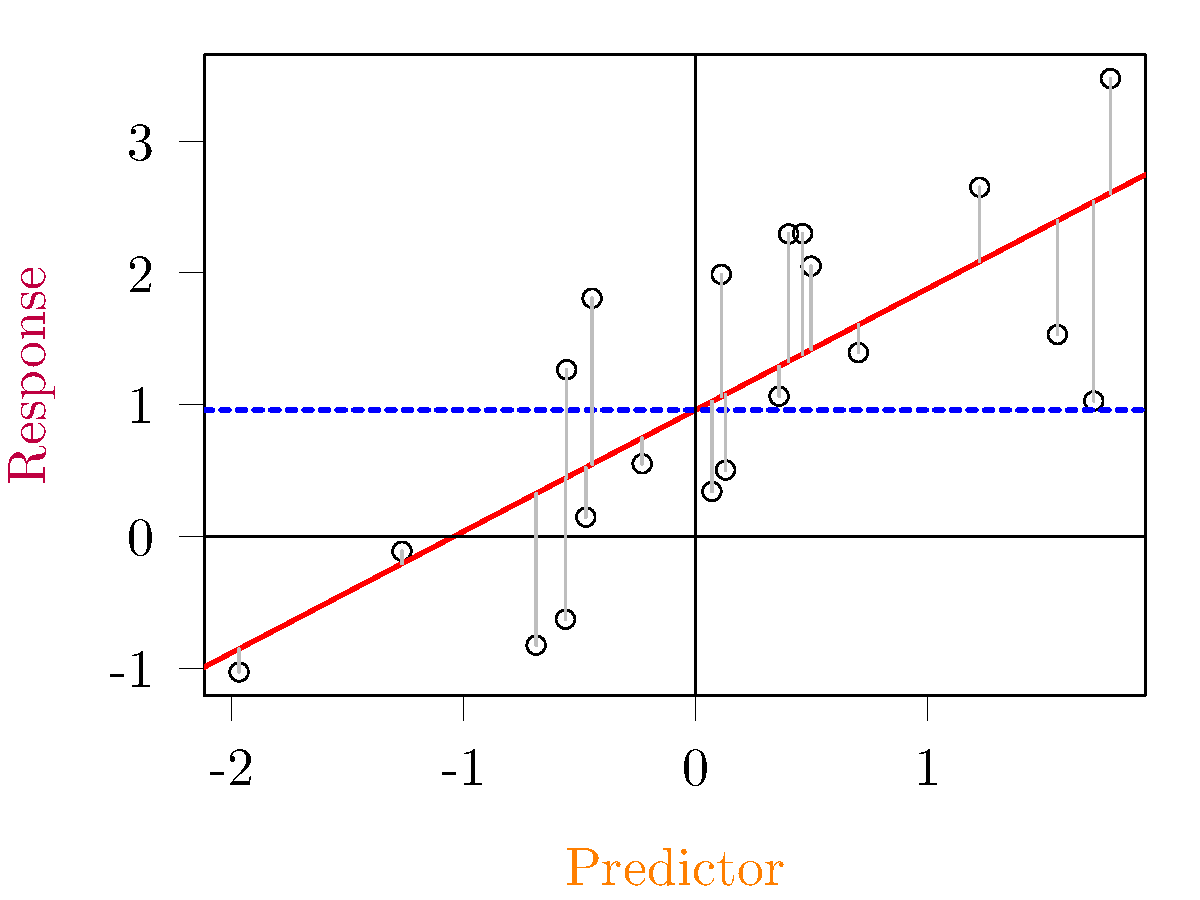
\includegraphics[width=0.6\textwidth]{Figures/lmprinc-1}

\only<1>{
$
\textbf{{\color{purple}{Response}} = {\color{blue}{Intercept}} + {\color{red}{Slope}} $\times$ {\color{orange}{Predictor}} }
$
}

\only<2->{
$
{\color{purple}{Response}} = \underbrace{{\color{blue}{Intercept}} + {\color{red}{Slope}} \times {\color{orange}{Predictor}}}_{\substack{\text{Mean Structure} \\ \text{Experimental factors}}} + \underbrace{{\color{gray}{Error}}, \text{ with } {\color{gray}{\epsilon \sim N(0,\sigma)}}}_{\substack{\text{Variance Structure} \\ \text{Unrelated to experiment factors} \\ \text{Unexplained ``noise''}}}
$
}

  \pause 
  \vfill
  
  What is in ${\color{gray}{\epsilon}}$? How can we tweak that? Why should we care?
  \end{frame}
%%%%%%%%%%%%

\begin{frame}{Let's do exercises in section 1}
 
\end{frame}
%%%%%%%%%%%%

\begin{frame}{Exercise 1:}

  \begin{columns}
    \begin{column}{0.5\textwidth}
	\begin{center}
	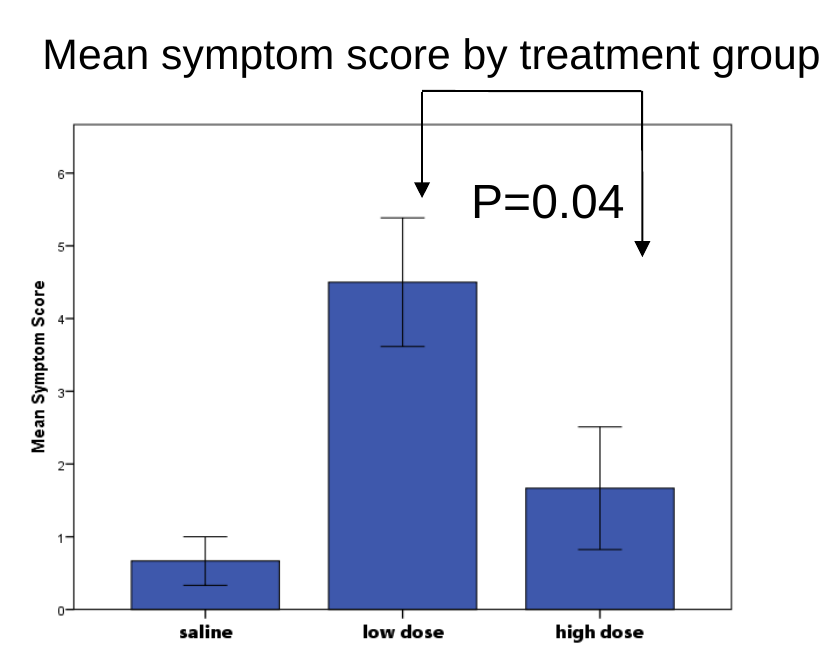
\includegraphics[width=\textwidth]{Figures/message1}
	\end{center}
    \end{column}
    
    \begin{column}{0.5\textwidth}
    \begin{block}{Vaccine challenge experiment:}
      \begin{itemize} 
       \item 6 mice/group (saline/low dose/high dose)
       \item All mice challenged with Shigella
       \item Followed for 14 days
       \item  Outcome: Symptom score average Days 2 - 8
      \end{itemize}
      \end{block}
      
      \begin{alertblock}{}
       One-way ANOVA (post-hoc Bonferroni) p=0.04
      \end{alertblock}

    \end{column}
  \end{columns}
  

\end{frame}
%%%%%%%%%%%%%%%%%%%%%%%


\begin{frame}{ Noise confounded with treatment}

 \begin{center}
  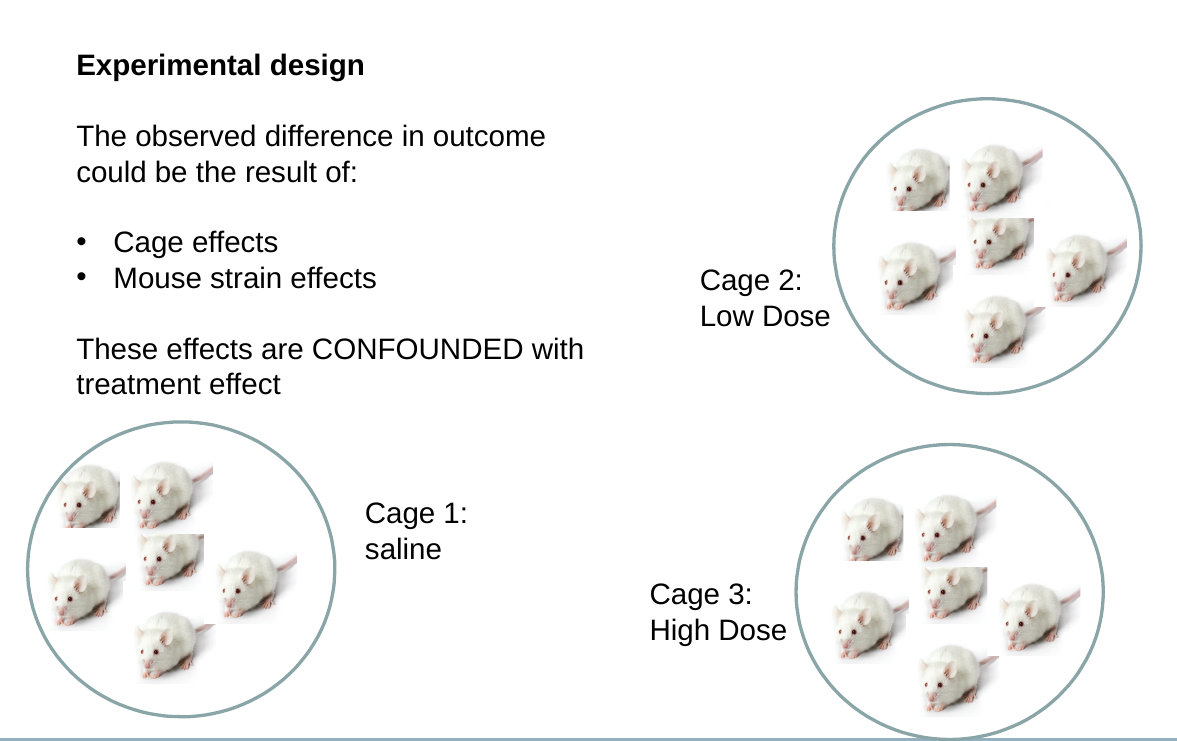
\includegraphics[width=0.7\textwidth]{Figures/mice}
 \end{center}
 
 \pause
 
 \begin{block}{Solutions:}
  Mixed cages: can compare within cages \\
  More cages: must compare between cages 
 \end{block}

\end{frame}
%%%%%%%%%%%

\begin{frame}{ Noise confounded with treatment}

  \begin{block}{Mixed cages: can compare within cages}
    \begin{itemize}
     \item \textbf{Share the noise among treatments}
     \item Few cages needed: Technically efficient
     \item But may be technically impossible
    \end{itemize}
  \end{block}

 \pause
 
 \begin{block}{More cages: must compare between cages }
    \begin{itemize}
    \item \textbf{Redefine experimental unit}
    \item Noise among cages, instead of within
    \item Needs to re-scale the experiment
    \end{itemize} 
 \end{block}

\end{frame}
%%%%%%%%%%%


\begin{frame}{Exercise 2:}
 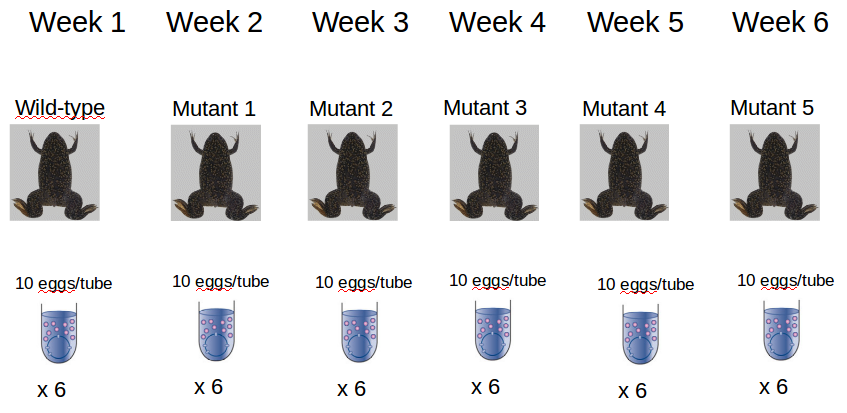
\includegraphics[width=\textwidth]{Figures/expdes2}
  
 \emph{\textbf{What is wrong with this design?}}
\end{frame}
%%%%%%%%%%%%

\begin{frame}{What is wrong with this design?}
 \begin{alertblock}{}
 \begin{itemize}
  \item CONTROLS: not tested under identical conditions
  \item REPLICATION: only pseudo-replication
  \item BLOCKING: none
  \item RANDOMISATION: NA
 \end{itemize}
 \end{alertblock}
 
 \pause
 
 \textbf{This experiment is useless}

\end{frame}
%%%%%%%%%%%%


\begin{frame}{What is going on conceptually?}
 $
{\color{purple}{Response}} = \underbrace{{\color{blue}{Intercept}} + {\color{red}{Slope}} \times {\color{orange}{Predictor}}}_{\substack{\text{Mean Structure} \\ \text{Experimental factors}}} + \underbrace{{\color{gray}{Error}}, \text{ with } {\color{gray}{\epsilon \sim N(0,\sigma)}}}_{\substack{\text{Variance Structure} \\ \text{Unrelated to experiment factors} \\ \text{Unexplained ``noise''}}}
$
\pause

\begin{alertblock}{For robust models we need assumptions about the error:}
 \begin{enumerate}
  \item Gaussian error distribution
  \item Homoscedasticity (constant error variance)
  \item \textbf{Independence of errors}
 \end{enumerate}
 
 That what $\epsilon \sim N(0,\sigma)$ means
\end{alertblock}

\pause

In mice and frog experiments, $\epsilon$ are non-independent

\end{frame}
%%%%%%%%%%%


%%%%%%%%%%%%%%%%%%%%%%%%%%%%%%%%%%%%%%%%%%%%%%%%%%%%%%%%%%%%%%%%
%%%%%%%%%%%%%%%%%%%%%%%%%%%%%%%%%%%%%%%%%%%%%%%%%%%%%%%%%%%%%%%%
%%%%%%%%%%%%%%%%%%%%%%%%%%%%%%%%%%%%%%%%%%%%%%%%%%%%%%%%%%%%%%%%



\begin{frame}{Fixed or random effect?}
  
  \begin{block}{In general}
   \begin{itemize}
    \item Doesn't change inference much. Random effect slightly more efficient.
    \item Summary cleaner with random effect, especially when many random levels
    \item Random shifts the focus from level values to variation among levels
    \item Variance parameters interesting in themselves
    \item Are levels of interest (fixed) or are they some kind of noise (random)
   \end{itemize}
  \end{block}

\end{frame}
%%%%%

\begin{frame}{Exercises with lme4 output}
 
\end{frame}
%%%%%%%%%%%


\begin{frame}{Understanding different variance structure}
 
 \begin{center}
  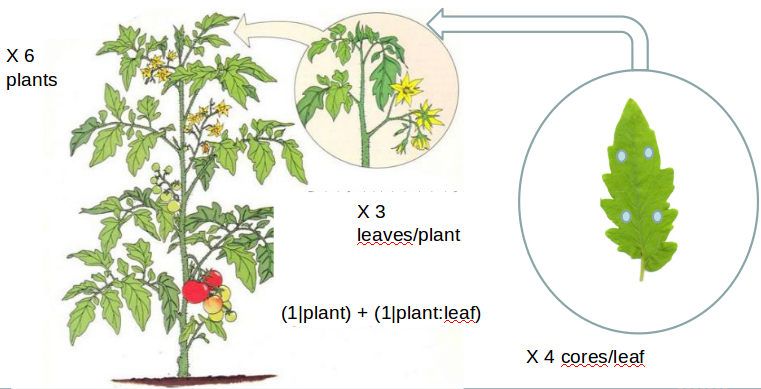
\includegraphics[width=0.9\textwidth]{Figures/nestedtomatoes}
 \end{center}

\end{frame}
%%%%%%%%%%%

\begin{frame}{Understanding different variance structure}
 
 \begin{center}
  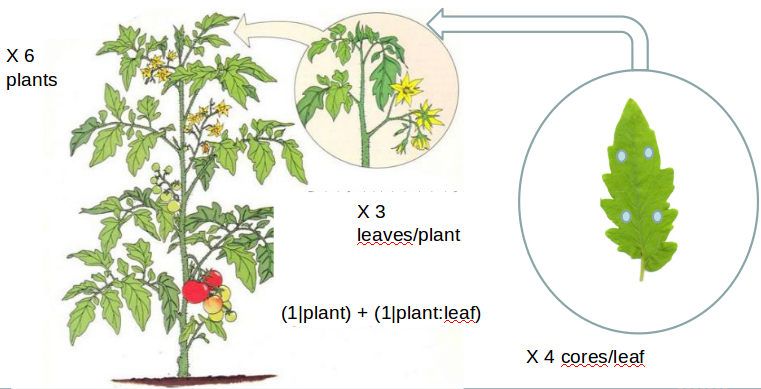
\includegraphics[width=0.9\textwidth]{Figures/nestedtomatoes}
 \end{center}

\end{frame}
%%%%%%%%%%%


\begin{frame}{Understanding different variance structure}
 
 \begin{center}
  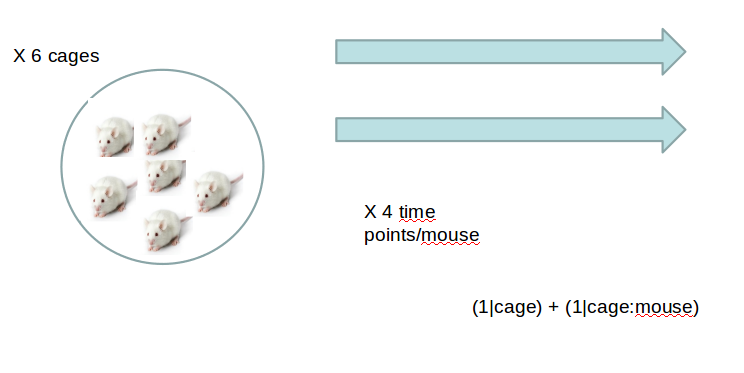
\includegraphics[width=0.9\textwidth]{Figures/nestedmice}
 \end{center}

\end{frame}
%%%%%%%%%%%



\begin{frame}{Understanding different variance structure: \textbf{Nested and Crossed structures}} 
\textbf{Crossed:} \texttt{(1|plate) + (1|row) + (1|column)}\\
\vspace{0.2cm}
\textbf{Nested:} \texttt{(1|plate) + (1|plate:row) + (1|plate:column) = (1|plate/row/column)}\\

What is the difference?

 \begin{center}
  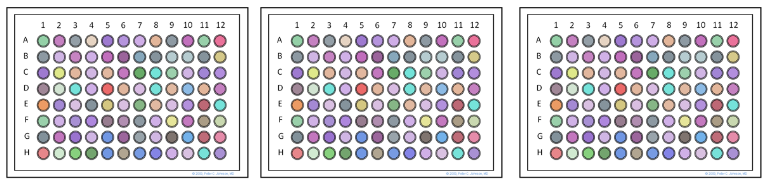
\includegraphics[width=0.9\textwidth]{Figures/nestedplates}
 \end{center}

 \textit{crossed random effects: one level of a random effect can appear in conjunction with more than one level of another random effect}
\end{frame}
%%%%%%%%%%%



\begin{frame}{Beyond random intercepts}


\begin{alertblock}{Right-hand side = what groups observations}
Nested, crossed et al. on the right hand side of the \texttt{|}: \texttt{(1|something)}\\
How are data related to each other, what groups them\\
Does not tell what parameter vary accoring to group
\end{alertblock}


\pause
\begin{alertblock}{Left-hand side = what varies according to grouping}
The \texttt{1} stands for \textbf{intercept}\\
But many things can go to the left hand side. 
\end{alertblock}

\pause

\begin{exampleblock}{Random interactions, random regressions, random slopes\dots}
 e.g., $y \sim 1 + x + (1 + x|something)$
\end{exampleblock}
 
\end{frame}
%%%%%%%%%%%



\begin{frame}{Everything you need to know about mixed models}

\begin{itemize}
 \item \url{http://bbolker.github.io/mixedmodels-misc/glmmFAQ.html}
 \item Subscribe to mailing-list: \texttt{https://stat.ethz.ch/mailman/listinfo/r-sig-mixed-models}
\end{itemize}

\end{frame}
%%%%%%%%%%%%%


\end{document}
